\documentclass{article}
\usepackage{graphicx}
\usepackage{amsmath}
\usepackage{pgfplots}
\usepackage{physics}
\usepackage{cancel}
\usepackage{enumitem}
\usepackage{txfonts}
\usepackage{multicol}

\pgfplotsset{compat=1.18}

\usepackage[a4paper, top=1cm, bottom=1cm, left=1cm, right=1cm, includehead, includefoot]{geometry}

\begin{document}

\noindent
Math 110B - Calculus \hfill Aaron W. Tarajos
\begin{center}
	\textbf{Final Exam Notes}
\end{center}

\noindent\rule{\textwidth}{0.4pt}

\begin{multicols}{2}

\subsubsection*{Trig angles}
    \begin{tabular}{|l|c|c|c|}
        \hline
	Function & $\frac{\pi}{4}(45)$ & $\frac{\pi}{3}(60)$ & $\frac{\pi}{6}(30)$\\
        \hline
	$\sin \theta$ & $\frac{2}{\sqrt2}$ & $\frac{\sqrt 3}{2}$ & $\frac{1}{2}$\\
	$\cos \theta$ & $\frac{2}{\sqrt2}$ & $\frac{1}{2}$ & $\frac{\sqrt{3}}{2}$ \\
	$\tan \theta$ & 1 & $\sqrt{3}$ & $\frac{\sqrt{3}}{3}$ \\
	\hline
    \end{tabular}

\subsubsection*{Work}
\[
	W = \int f(x)\ dx \quad OR \quad W = \int \rho \cdot d \cdot A \ dy
\]

\subsubsection*{Integration by parts}
\[
	\int f(x)g^\prime(x)\ dx = \int f(x)g(x) - \int g(x)f^\prime(x)\ dx
\]

\subsubsection*{Partial Fraction Decomposition}
Given some rational function
\[
	\frac{x+1}{(x+1)(x+3)} = \frac{A}{x+1} + \frac{B}{x+3} \implies x+1 = A(x+3) + B(x+1)
\]
Solve for A and B using a system of equations then integrate. Note if we have a repeat term like $(x+1)^2$ then;
\[
	\frac{x+1}{(x+1)^2(x+3)} = \frac{A}{x+1} + \frac{B}{(x+1)^2} + \frac{C}{x+3}
\]
Then solve as normal

\subsubsection*{Volumes by slices}
\[
	V = \int_{x_1}^{x_2} \pi r^2(x)\ dx \quad \text{OR} \quad V = \int_{x_1}^{x^2} \pi \left(r_1^2 - r_2^2 \right)\ dx
\]

\subsubsection*{Volumes by shells}
\[
	V = \int_{x_1}^{x_2} 2\pi x f(x)\ dx
\]
Note: be careful about the integration bounds and radius, for example,  a slice with $r_1$ of $y=3$ and $r_2$ of $\sec(x) + 1$ rotated about $y=1$ would be\\ $A = \pi \left( (3-1)^2 - (\sec(x) + 1 - 1)^2 \right)$.

\subsubsection*{Trig sub}
\begin{minipage}{0.2\textwidth}
    \begin{tabular}{|l|l|}
        \hline
        Expression & Substitution\\
        \hline
        $\sqrt{a^2-x^2}$ & $x=a\sin\theta$\\
        $\sqrt{a^2+x^2}$ & $x=a\tan\theta$\\
        $\sqrt{x^2-a^2}$ & $x=a\sec\theta$\\
        \hline
    \end{tabular}
\end{minipage}
\begin{minipage}{0.3\textwidth}
    \begin{enumerate}
	\item Draw a triangle
	\item Define the edge lengths using pythagorean theorem
	\item Define trig functions for the triangle
	\item Sovle for $x$ in terms of a trig function and $dx$. Ex;
		\[
			x = \sin \theta (x)
		\]
		\[
			dx = cos \theta\ d \theta
		\]
    \end{enumerate}
\end{minipage}

\subsubsection*{Arc length}
\[
	L = \int_a^b \sqrt{1 + \left(\frac{dy}{dx}\right)^2}\ dx
\]
Derived from pathagorean theorem for the infinite sum of secant lines i.e. $\sqrt{\Delta x^2 + \Delta y^2} = \sqrt{\Delta x^2 + (f^\prime(x)\Delta x)^2}$ factor out $\Delta x$ to obtain the equation.

\subsubsection*{Some other useful antiderivates}
\begin{align*}
	\int \frac{1}{\sqrt{1-x^2}} &= \arcsin x + C \\
	\int -\frac{1}{\sqrt{1-x^2}} &= \arccos x + C \\
	\int \frac{dx}{x^2-a^2} &= \frac{1}{2a} \ln \left| \frac{x-a}{x+a} \right| \\
	\int \frac{dx}{\sqrt{x^2 \pm a^2}} &= \ln \left| x + \sqrt{x^2 \pm a^2} \right| \\
\end{align*}

\subsubsection*{Surface area}
\[
	S = 2\pi \int_a^b y \sqrt{1+\left( \frac{dy}{dx} \right)^2}\ dx
\]

\subsubsection*{Hydrostatic force}
Pressure is given by
\[
	P = \int_\text{deepest point}^\text{shallow point} \rho \cdot area \cdot depth
\]

where area is width as a function of y and height is $dy$ and $\rho$ is the density.

\subsubsection*{Trig integral tip}
If encountering a form like
\[
	\int \sin^5 x \cos^4 x\ dx
\]
let $u$ be the lower order term and keep one of the higher order terms from the other then convert the rest to match using $1 = \cos^2 x + \sin^2 x$

\end{multicols}

\pagebreak
\subsection*{Problems that were implied to be on the exam}
\begin{multicols}{2}
\subsubsection*{Separable differential equation with PFD}
\begin{align*}
	\frac{dy}{dx} &= y \cdot \frac{x+1}{(x-1)^2(x+2)} \\
	\frac{1}{y} \frac{dy}{dx} &= \frac{x+1}{(x-1)^2(x+2)} \\
	\int \frac{1}{y} \frac{dy}{dx}\ dx &= \int \frac{x+1}{(x-1)^2(x+2)}\ dx \\
	& \text{by ROS} \\
	\int \frac{1}{y}\ dy &= \int \frac{x+1}{(x-1)^2(x+2)}\ dx
\end{align*}
handling the fraction;
\begin{align*}
\frac{x+1}{(x-1)^2(x+2)} &= \frac{A}{(x-1)^2} + \frac{B}{x+2} + \frac{C}{x-1} \\
	x + 1 &= A(x+2) + B(x-1)^2 + C(x-1)(x+2) \\
	x + 1 &= Ax + 2A + Bx^2 -2Bx + B + Cx^2 + Cx -2C \\
	x + 1 &= x(A-2B+C) + x^2(B+C) + (2A + B - 2C)
\end{align*}
then we have the system of equations;
\begin{align*}
	0 &= B+C \\
	1 &= 2A + B-2C \\
	1 &= A - 2B + C
\end{align*}
\[
	2 = 3A \implies A = \frac{2}{3}
\]
Solve for $B$ and $C$ we obtain the following
\begin{align*}
	\int \frac{1}{y}\ dy &= \int \left( \frac{2/3}{(x-1)^2} + \frac{-1/9}{x+2} + \frac{1/9}{x-1} \right)\ dx
\end{align*}
Use $u$-sub on the first term where $u = x-1$;
\[
	\frac{2}{3} \int \frac{1}{u^2} = -\frac{2}{3u}
\]
so we have;
\[
	\ln|y| = \frac{2}{3x-3} + \frac{1}{9}\ln|x-1| -\frac{1}{9}\ln|x+2| + C
\]

\subsubsection*{Improper integrals}
\begin{align*}
	\int_{-3}^2 \frac{1}{6+2x}\ dx &= \lim_{a \to -3} \int_a^2 \frac{1}{6+2x}\ dx \\
				       &= \lim_{a \to -3} \left[ \frac{\ln|2x+6|}{2} \right]_a^2 \\
				       &= \lim_{a \to -3} \frac{\ln|2(2)+6|}{2} - \lim_{a \to -3} \frac{\ln|2(a)+6|}{2}
\end{align*}
the limit is undefined therefore the integral is divergent.

\subsubsection*{Revolution}
Find the volume of the region bounded by
\[
	y = x^2 -6x +9 \quad \text{and} \quad y=-x^2 +6x -1
\]
rotated about $x=8$. These are two parabolas, find the horizontal integration bounds by setting them equaal to eachother and solving for $x$. Then find the vertex by finding the critical points by setting derivative to zero and solving. Height as a function of $x$ is the difference between the two functions, radius is $8 - x$.

\subsubsection*{Trig sub + u-sub}
\[
	\int_{-7}^{4} \frac{1}{t^4 \sqrt{t^2-25}}\ dt
\]

\begin{center}
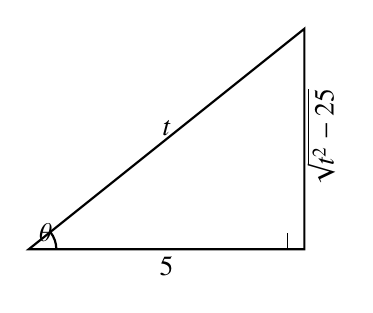
\begin{tikzpicture}[scale=0.7]
    % Draw the triangle
    \draw[thick] (0, 0) -- (5, 0) -- (5, 4) -- cycle;

    % Label the sides
    \node at (2.5, -0.3) {5}; % Adjacent side
    \node[rotate=90] at (5.3, 2) {\(\sqrt{t^2-25}\)}; % Opposite side
    \node at (2.5, 2.2) {\(t\)}; % Hypotenuse

    % Label the angle
    \node at (0.3, 0.3) {\(\theta\)};

    % Mark the angle
    \draw[thick] (0.5, 0) arc[start angle=0, end angle=38, radius=0.5];

    % Right angle symbol
    \draw (5, 0) -- ++(-0.3, 0) -- ++(0, 0.3);
\end{tikzpicture}
\end{center}

\begin{align*}
	\sec \theta &= \frac{t}{5} \\
	\tan \theta &= \frac{\sqrt{t^2-25}}{5} \\
	\frac{d}{dt} 5 \sec \theta &= \frac{d}{dt} t \implies 5 \sec \theta \tan \theta \frac{d \theta}{dt} = 1
\end{align*}
then make our substitutions;
\begin{align*}
	\int_{-7}^{4} &\frac{1}{5^4 \sec^4 \theta} \cdot \frac{1}{5 \tan \theta} 5\sec\theta\tan\theta \frac{d \theta}{dt}\ dt \\
	&= \frac{1}{5^4} \cdot \frac{1}{sec^3 \theta} \frac{d \theta}{dt}\ dt \\
	& \text{by ROS} \\
	&= \frac{1}{5^4} \int_A^B \cos^3\theta\ d \theta \\
	&= \frac{1}{5^4} \int_A^B (1-\sin^2 \theta) \cos\theta\ d \theta \\
	&\text{let $u = \sin \theta$} \\
	...
\end{align*}


\subsubsection*{Taylor series}
Find T$_4(x)$ for $x$ near $x=1$ for the function
\[
	f(x) = \ln (1+2x)
\]

\begin{align*}
	f^\prime(x) &= \frac{1}{2x+1} \cdot 2 \biggr\vert_{x=1} = \frac{2}{3} \\
	f^{\prime \prime}(x) &= -\frac{2^2}{(2x+1)^2} \biggr\vert_{x=1} = \frac{2^2}{3^2} \\
	f^{\prime \prime \prime}(x) &= \frac{2^4}{(2x+1)^3} \biggr\vert_{x=1} = \frac{2^4}{3^3}\\
	f^{\prime \prime \prime \prime}(x) &= -\frac{2^5 \cdot 3}{(2x+1)^4} \biggr\vert_{x=1} = \frac{2^5}{3^3}
\end{align*}
The use Talor's formula;
\[
	f(a) + \frac{f^\prime(a)}{1!}(x-a) + \frac{f^{\prime \prime}(a)}{2!}(x-a)^2 + \frac{f^{\prime \prime \prime}(a)}{3!}(x-a)^3 + \dots
\]

\subsubsection*{Power Series Integral}
Evaluate the following integral using a power series;
\[
	\int \frac{1}{1+x^6}\ dx
\]
We know that
\[
	1 + x + x^2 + x^3 + \dots = \frac{1}{1-x}
\]
therefore
\[
	1 + (-x^6) + (-x^6)^2 + (-x^6)^3 + \dots = \frac{1}{1+x^6}
\]
and
\begin{align*}
	\int 1-x^6+x^{12}-x^{18} + \dots \ dx &= x - \frac{x^7}{7}+\frac{x^13}{13}-\frac{x^19}{19} + \dots \\
	&= \sum_{n=0}^\infty (-1)^n \frac{ x^{6n+1}}{6n+1} + C
\end{align*}

\subsubsection*{Convergence tests}
Is the series absolutely convergent, conditionally convergent, or divergent;
\[
	\sum_{n=1}^\infty (-1)^n \frac{\ln n}{\sqrt{n}}
\]
absolute convergence:
\[
	\sum_{n=1}^\infty \Biggr\vert (-1)^n \frac{\ln n}{\sqrt{n}} \Biggr\vert = \sum_{n=1}^\infty \frac{\ln n}{\sqrt{n}}
\]
Comparison test
for power series it converges for $p > 1$ and diverges for $p \le 1$. We know that $\frac{ln n}{\sqrt{n}} > \frac{1}{\sqrt{n}}$ for $n>3$ so we can check
\[
	\sum = \frac{1}{n^p}
\]
and because
\[
	\sum_{n=1}^\infty = \frac{1}{n^{1/2}}
\]
we say that by the comparison test the series is divergent. Now check conditional convergence, alternating series test; is the function decreasing?
\[
	f^\prime(x) = \frac{\sqrt{x}/x - \ln x \frac{1}{2\sqrt{x}}}{\sqrt{x}^2} = \frac{2-\ln x}{2x^{3/2}}
\]
which is decreasing for $x > e^2$. Now we check that the limit approaches 0.
\[
	\lim_{n \to \infty} \frac{\ln n}{\sqrt{n}} \quad \text{idet.}\ \frac{\infty}{\infty}
\]
Using L'H;
\[
	\lim_{n \to \infty} \frac{2}{\sqrt{n}} = 0
\]
Therefore the series converges conditionally

\subsubsection*{Notable tricks if you're stuck}
\begin{enumerate}
	\item You can integrate by parts with $g(x) = 1$
	\item \[ \frac{x^2}{x^2+1} = \frac{x^2 + 1 - 1}{x^2 +1} = 1 - \frac{1}{x^2+1} \]
	\item related to (2) find creative ways to multiply by 1 to create substitutable problems. i.e. $\int \sec \theta$ see below
	\item when doing $u$ sub you can write $x$ as a function of $u$ and sub out remaining $x$ that are unresolved by $\frac{du}{dx}$
	\item for absolute value setup as piecewise and integrate both sides of zero.
\end{enumerate}

\begin{align*}
	\int \sec \theta \ d \theta &= \int \sec \theta \cdot \frac{\sec \theta + \tan \theta}{\sec \theta + \tan \theta} \ d \theta \\
				    &= \int \frac{sec^2 \theta + \sec \theta \tan \theta}{\sec \theta + \tan \theta} \ d \theta \\
				    &= \int \frac{1}{u} \ du \\
				    &= \ln|u| \\
				    &= \ln|\sec \theta + \tan \theta | + C
\end{align*}

\subsubsection*{Series Tests}
Alternating series;
\[
	\sum (-1)^{n-1} b_n = b_1 - b_2 + b_3 - b_4 +\dots
\]
if $b_{n+1} > n$ for all $n$ and if $\lim_{n \to \infty} b_n = 0$ then the series is convergent.\\
Ration test;
\[
	\lim_{n \to \infty} \Biggr\vert \frac{a_{n+1}}{a_n} \Biggr\vert
\]
if the limit is $< 1$ absolutely convergent if $> 1$ divergent.\\
Root test;
\[
	\lim_{n \to \infty} \sqrt[n]{|a_n|}
\]
same conditions as ratio test.

\end{multicols}

\end{document}
